\section{Proposed Approach}
\label{sec: approach}
In this section, we present our method of probabilistic Gaussian superposition for efficient 3D semantic occupancy prediction.
We first review the original 3D semantic Gaussian representation~\cite{huang2024gaussian} and its limitations (Sec.~\ref{subsec: old gaussian}).
We then introduce our probabilistic Gaussian modeling and how we derive geometry and semantics predictions based on the multiplication theorem of probability and Gaussian mixture model (Sec.~\ref{subsec: prob modeling}).
Finally, we detail the distribution-based initialization module to effectively initialize probabilistic Gaussians around the occupied area (Sec.~\ref{subsec: initialization}).


\subsection{3D Semantic Gaussian Representation}
\label{subsec: old gaussian}
Vision-centric 3D semantic occupancy prediction~\cite{cao2022monoscene,huang2023tri} aims to obtain the fine-grained geometry and semantics of the 3D scene.
To formulate, the target is to predict voxel-level semantic segmentation result $\mathbf{O}\in \mathcal{C}^{X\times Y\times Z}$ given input images $\mathcal{I}=\{\mathbf{I}_i\}_{i=1}^{N}$, where $\mathcal{C}$, $\{X, Y, Z\}$, $N$ represent the set of predefined classes, the spatial resolution of occupancy and the number of input views, respectively.

To achieve this, 3D semantic Gaussian representation employs a set of $P$ Gaussian primitives $\mathcal{G}=\{\mathbf{G}_i\}_{i=1}^{P}$, with each $\mathbf{G}_i$ describing a local region with its mean $\mathbf{m}_i$, scale $\mathbf{s}_i$, rotation $\mathbf{r}_i$, opacity $a_i$ and semantics $\mathbf{c}_i$.
GaussianFormer interprets these primitives as local semantic Gaussian distributions which contribute to the overall occupancy prediction through additive aggregation:
\vspace{-2mm}
\begin{equation}
    \hat{\mathbf{o}}(\mathbf{x}; \mathcal{G})=\sum_{i=1}^{P}\mathbf{g}_i(\mathbf{x}; \mathbf{m}_i,\mathbf{s}_i,\mathbf{r}_i,a_i,\mathbf{c}_i),
    \label{eq: weighted summation}
    \vspace{-2mm}
\end{equation}
where $\mathbf{g}_i(\mathbf{x};\cdot)$ denotes the contribution of the $i$th semantic Gaussian to $\hat{\mathbf{o}}(\mathbf{x}; \mathcal{G})$ which is the overall occupancy prediction at location $\mathbf{x}$.
The contribution $\mathbf{g}$ is further calculated as the corresponding semantic Gaussian distribution evaluated at location $\mathbf{x}$:
\begin{equation}
    \mathbf{g}(\mathbf{x}; \mathbf{G}) = a\cdot{\rm{exp}}\big(-\frac{1}{2}(\mathbf{x}-\mathbf{m})^{\rm T} \mathbf{\Sigma}^{-1} (\mathbf{x}-\mathbf{m})\big)\mathbf{c},
    \label{eq: gaussian dist}
\end{equation}
\begin{equation}
    \mathbf{\Sigma} = \mathbf{R}\mathbf{S}\mathbf{S}^T\mathbf{R}^T, \quad \mathbf{S} = {\rm{diag}}(\mathbf{s}), \quad \mathbf{R} = {\rm{q2r}}(\mathbf{r}),
\end{equation}
where $\mathbf{\Sigma}$, $\mathbf{R}$, $\mathbf{S}$ represent the covariance matrix, the rotation matrix constructed from the quaternion $\mathbf{r}$ with function ${\rm q2r}(\cdot)$, and the diagonal scale matrix from function ${\rm diag}(\cdot)$.

Although the number of Gaussians is reduced compared with the number of dense voxels thanks to the deformable nature of Gaussian distributions as in Eq.~(\ref{eq: gaussian dist}), several limitations still persist in the 3D semantic Gaussian representation.
First of all, it models both the occupied and unoccupied regions in the same way using the semantic property $\mathbf{c}$, resulting in most Gaussians being classified as empty given the huge proportion of empty space in outdoor scenarios.
Secondly, the semantic Gaussian representation encourages Gaussians to overlap, because the aggregation process in Eq.~(\ref{eq: weighted summation}) independently sums up the contribution of each Gaussian, resulting in unbounded occupancy prediction $\hat{\mathbf{o}}$.
For optimization, the model would learn to allocate more Gaussians to describe the same region due to the unbounded nature of $\hat{\mathbf{o}}$, aggravating the overlap between Gaussians.
These limitations stem from the current interpretation of Gaussians and obstruct the efficiency and effectiveness of the 3D semantic Gaussian representation.
Our method approaches Gaussian-based object-centric representation from a probabilistic perspective, serving as a fundamental solution to these issues, as shown by Figure~\ref{fig:motivation}.


\subsection{Probabilistic Gaussian Superposition}
\label{subsec: prob modeling}
We propose the probabilistic Gaussian superposition as an efficient and effective 3D scene representation.
As shown in Figure~\ref{fig:pipeline}, we decompose the 3D modeling target into geometry and semantics predictions, and adopt the multiplication theorem of probability and the Gaussian mixture model to address them from a probabilistic perspective, respectively.

\textbf{Geometry prediction.}
To restrict Gaussians to represent only occupied regions for geometry prediction, we interpret the Gaussian primitives $\mathcal{G}=\{\mathbf{G}_i\}_{i=1}^{P}$ as the probability of their surrounding space being occupied.
To elaborate, we assign a probability value of 100\% at the centers of Gaussians, which decays exponentially with respect to the distance from the centers $\mathbf{m}$:
\begin{equation}
    \alpha(\mathbf{x};\mathbf{G}) = {\rm{exp}}\big(-\frac{1}{2}(\mathbf{x}-\mathbf{m})^{\rm T} \mathbf{\Sigma}^{-1} (\mathbf{x}-\mathbf{m})\big),
    \label{eq: single prob}
\end{equation}
where $\alpha(\mathbf{x};\mathbf{G})$ denotes the probability of the point $\mathbf{x}$ being occupied induced by Gaussian $\mathbf{G}$.
Eq.~(\ref{eq: single prob}) assigns a high probability of occupancy when the point $\mathbf{x}$ is close to the center of Gaussian $\mathbf{G}$, which prevents any Gaussian from describing empty area.
To further derive the overall probability of occupancy, we assume that the probabilities of a point being occupied by different Gaussians are mutually independent, and thus we can aggregate them according to the multiplication theorem of probability:
\vspace{-1mm}
\begin{equation}
    \alpha(\mathbf{x}) = 1 - \prod_{i=1}^{P}\big(1 - \alpha(\mathbf{x};\mathbf{G}_i)\big),
    \label{eq: multi prob}
    \vspace{-1mm}
\end{equation}
where $\alpha(\mathbf{x})$ represents the overall probability of occupancy at point $\mathbf{x}$. 
In addition to achieving object-centric properties, Eq.~(\ref{eq: multi prob}) also avoids unnecessary overlapping between Gaussians because $\alpha(\mathbf{x}) \ge \alpha(\mathbf{x};\mathbf{G}_i)$ holds for any Gaussian $\mathbf{G}_i$.
This implies that point $\mathbf{x}$ would be predicted occupied if it is close enough to any single Gaussian.


\textbf{Semantics prediction.}
In addition to object-centric anti-overlapping geometry modeling, we still need to achieve the same goals for semantics prediction.
We first remove the channel that represents the empty class from the semantic properties $\mathbf{c}$ of Gaussians since it has been accounted for in geometry prediction.
Then we interpret the set of Gaussians $\mathcal{G}$ as a Gaussian mixture model, where semantics prediction could be formulated as calculating the expectation of semantics given the probabilistic Gaussian mixture model.
Specifically, we take the original opacity properties $a$ as the prior distribution of Gaussians, which is $l^1$-normalized.
Furthermore, we adopt the Gaussian probabilistic distribution parameterized by mean $\mathbf{m}$, scale $\mathbf{s}$ and rotation $\mathbf{r}$ as the conditional probability.
Then we normalize the original semantics properties $\mathbf{c}$ with softmax to ensure the boundedness of predicted semantics.
Finally, we calculate the expectation $\mathbf{e}(\mathbf{x};\mathcal{G})$ as:
\vspace{-1mm}
\begin{equation}
\begin{aligned}
    \mathbf{e}(\mathbf{x};\mathcal{G}) &= \sum_{i=1}^{P} p(\mathbf{G}_i|\mathbf{x})\Tilde{\mathbf{c}}_i 
    = \frac{\sum_{i=1}^{P}p(\mathbf{x}|\mathbf{G}_i)a_i\Tilde{\mathbf{c}}_i}{\sum_{j=1}^{P}p(\mathbf{x}|\mathbf{G}_j)a_j},
\end{aligned}
\label{eq: gmm}
\end{equation}
\begin{small}
\begin{equation}
    p(\mathbf{x}|\mathbf{G}_i) = \frac{1}{(2\pi)^{\frac{3}{2}}|\mathbf{\Sigma}|^{\frac{1}{2}}}{\rm{exp}}\big(-\frac{1}{2}(\mathbf{x}-\mathbf{m})^{\rm T} \mathbf{\Sigma}^{-1} (\mathbf{x}-\mathbf{m})\big),
\end{equation}
\end{small}where $p(\mathbf{G}_i|\mathbf{x})$, $p(\mathbf{x}|\mathbf{G}_i)$ and $\Tilde{\mathbf{c}}_i$ denote the posterior probability of point $\mathbf{x}$ belonging to the $i$th Gaussian distribution, the conditional probability of point $\mathbf{x}$ given the $i$th Gaussian distribution, and the softmax-normalized semantic properties, respectively. 
Compared with Eq.~(\ref{eq: weighted summation})(\ref{eq: gaussian dist}), the gaussian mixture model in Eq.~(\ref{eq: gmm}) normalizes the semantic properties and the contributions from different Gaussians, thus preventing unnecessary overlapping between Gaussians and producing normalized class probabilities directly.

Given the geometry and semantics predictions, we take a simple step forward to combine them to generate the final semantic occupancy prediction:
\begin{equation}
    \hat{\mathbf{o}}(\mathbf{x};\mathcal{G}) = [1-\alpha(\mathbf{x}); \alpha(\mathbf{x})\cdot\mathbf{e}(\mathbf{x};\mathcal{G})],
    \label{eq: final occ}
\end{equation}
where we use the geometry probability $\alpha(\mathbf{x})$ to weight the semantic predictions, and directly take $1 - \alpha(\mathbf{x})$ as the probability of the empty class.

\begin{figure}[t]
\centering
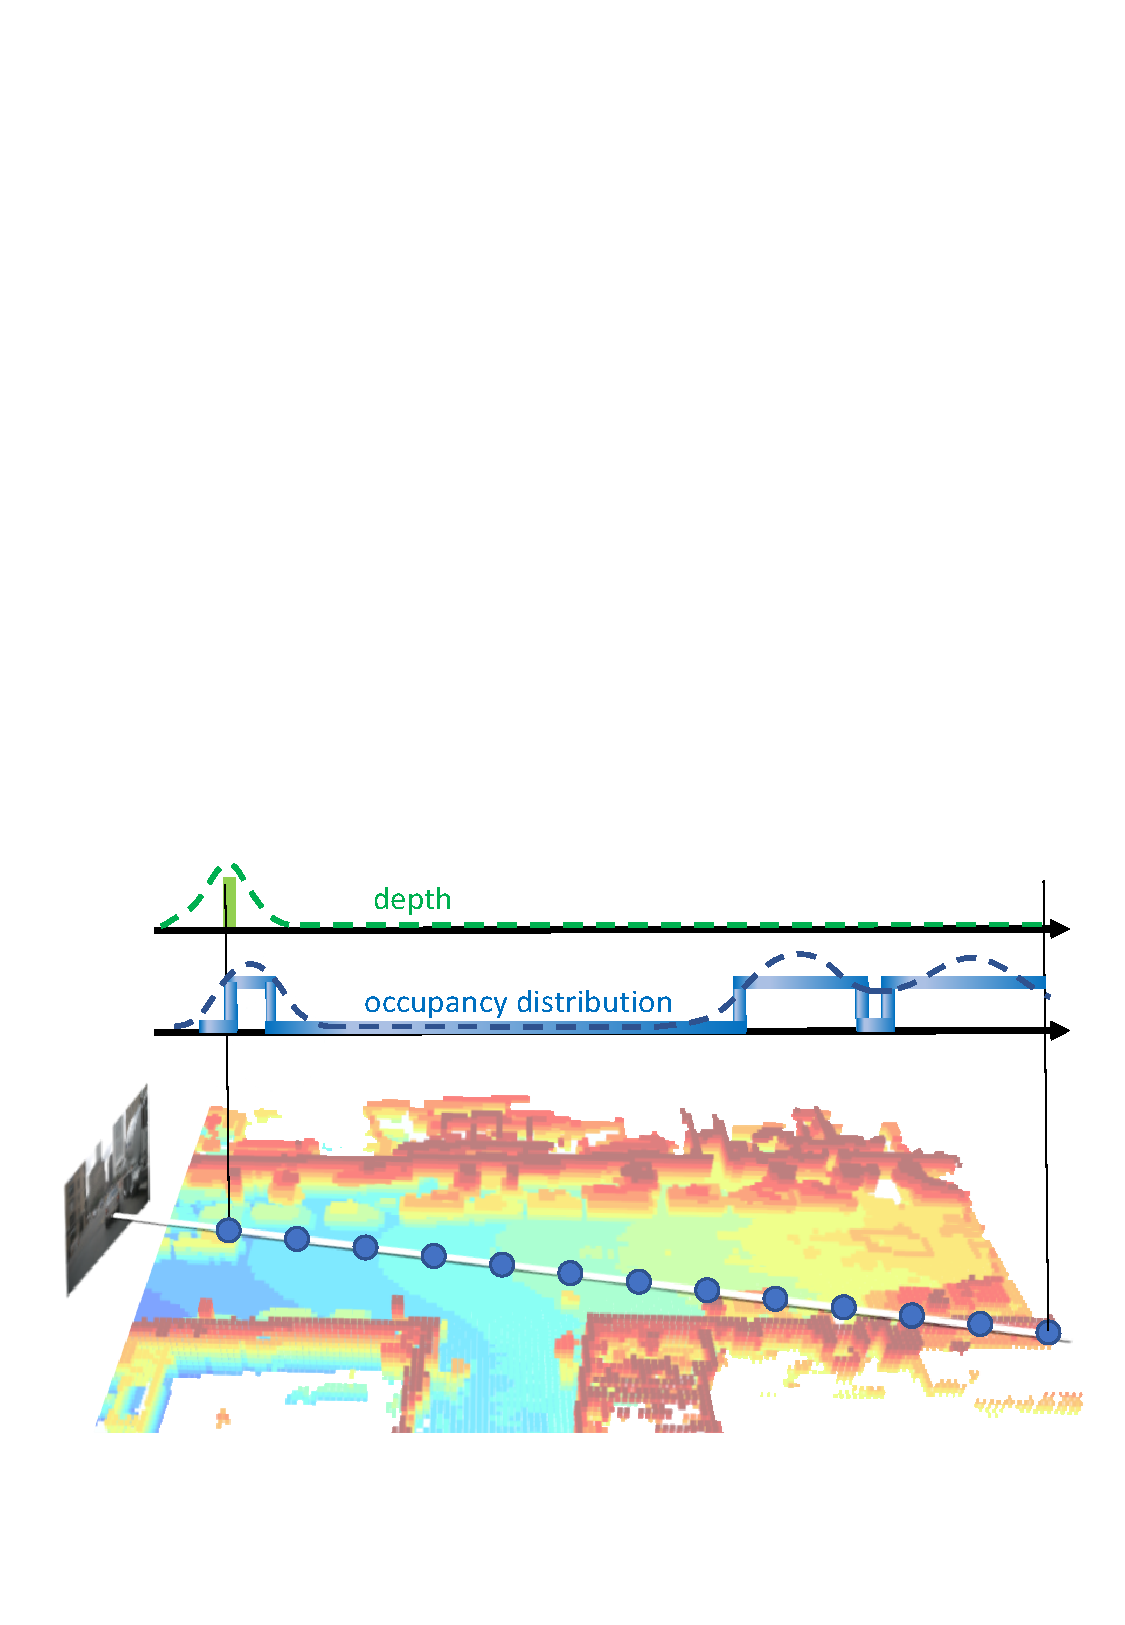
\includegraphics[width=0.95\linewidth]{figures/initialization.pdf}
\vspace{-2mm}
\caption{\textbf{Distribution-based initialization.}
Our initialization scheme learns pixel-aligned occupancy distributions from occupancy annotation, while the depth-based counterpart only captures the surfaces of objects and relies on LiDAR supervision.
}
\label{fig:initialization}
\vspace{-6mm}
\end{figure}

\begin{table*}[t] %
    \caption{\textbf{Surround view 3D semantic occupancy prediction results on nuScenes.} 
    * means supervised by dense occupancy annotations as opposed to original LiDAR segmentation labels.
    Ch. denotes the channel dimension of our model.
    Our method achieves state-of-the-art performance compared with other methods.}
    \small
    \setlength{\tabcolsep}{0.005\linewidth}  
    \vspace{-3mm}  
    \renewcommand\arraystretch{1.05}
    \centering
    \resizebox{\textwidth}{!}{
    \begin{tabular}{l|c c | c c c c c c c c c c c c c c c c}
        \toprule
        Method
        & IoU
        & mIoU
        & \rotatebox{90}{\textcolor{nbarrier}{$\blacksquare$} barrier}
        & \rotatebox{90}{\textcolor{nbicycle}{$\blacksquare$} bicycle}
        & \rotatebox{90}{\textcolor{nbus}{$\blacksquare$} bus}
        & \rotatebox{90}{\textcolor{ncar}{$\blacksquare$} car}
        & \rotatebox{90}{\textcolor{nconstruct}{$\blacksquare$} const. veh.}
        & \rotatebox{90}{\textcolor{nmotor}{$\blacksquare$} motorcycle}
        & \rotatebox{90}{\textcolor{npedestrian}{$\blacksquare$} pedestrian}
        & \rotatebox{90}{\textcolor{ntraffic}{$\blacksquare$} traffic cone}
        & \rotatebox{90}{\textcolor{ntrailer}{$\blacksquare$} trailer}
        & \rotatebox{90}{\textcolor{ntruck}{$\blacksquare$} truck}
        & \rotatebox{90}{\textcolor{ndriveable}{$\blacksquare$} drive. suf.}
        & \rotatebox{90}{\textcolor{nother}{$\blacksquare$} other flat}
        & \rotatebox{90}{\textcolor{nsidewalk}{$\blacksquare$} sidewalk}
        & \rotatebox{90}{\textcolor{nterrain}{$\blacksquare$} terrain}
        & \rotatebox{90}{\textcolor{nmanmade}{$\blacksquare$} manmade}
        & \rotatebox{90}{\textcolor{nvegetation}{$\blacksquare$} vegetation}
        \\
        \midrule
        MonoScene~\cite{cao2022monoscene} & 23.96 & 7.31 & 4.03 &	0.35& 8.00& 8.04&	2.90& 0.28& 1.16&	0.67&	4.01& 4.35&	27.72&	5.20& 15.13&	11.29&	9.03&	14.86 \\
        
        Atlas~\cite{murez2020atlas} & 28.66 & 15.00 & 10.64&	5.68&	19.66& 24.94& 8.90&	8.84&	6.47& 3.28&	10.42&	16.21&	34.86&	15.46&	21.89&	20.95&	11.21&	20.54 \\
        
        BEVFormer~\cite{li2022bevformer} & 30.50 & 16.75 & 14.22 &	6.58 & 23.46 & 28.28& 8.66 &10.77& 6.64& 4.05& 11.20&	17.78 & 37.28 & 18.00 & 22.88 & 22.17 & {13.80} &	\textbf{22.21}\\
        
        TPVFormer~\cite{huang2023tri} & 11.51 & 11.66 & 16.14&	7.17& 22.63	& 17.13 & 8.83 & 11.39 & 10.46 & 8.23&	9.43 & 17.02 & 8.07 & 13.64 & 13.85 & 10.34 & 4.90 & 7.37\\
        
        TPVFormer*~\cite{huang2023tri}  & {30.86} & 17.10 & 15.96&	 5.31& 23.86	& 27.32 & 9.79 & 8.74 & 7.09 & 5.20& 10.97 & 19.22 & {38.87} & {21.25} & {24.26} & {23.15} & 11.73 & 20.81\\

        OccFormer~\cite{zhang2023occformer} & {31.39} & {19.03} & {18.65} & {10.41} & {23.92} & {30.29} & {10.31} & {14.19} & {13.59} & {10.13} & {12.49} & {20.77} & {38.78} & 19.79 & 24.19 & 22.21 & {13.48} & {21.35}\\
        
        SurroundOcc~\cite{wei2023surroundocc} & {31.49} & {20.30}  & {20.59} & {11.68} & {28.06} & \textbf{30.86} & {10.70} & {15.14} & \textbf{14.09} & \textbf{12.06} & \textbf{14.38} & {22.26} & 37.29 & {23.70} & {24.49} & {22.77} & \textbf{14.89} & {21.86}  \\


        GaussianFormer~\cite{huang2024gaussian} & 29.83 & {19.10} & {19.52} & {11.26} & {26.11} & {29.78} & {10.47} & {13.83} & {12.58} & {8.67} & {12.74} & {21.57} & {39.63} & {23.28} & {24.46} & {22.99} & 9.59 & 19.12 \\

        \midrule
        \textbf{Ours} (Ch. = 128) & 30.56 & 20.02 & 20.15 & 12.99 & 27.61 & 30.23 & \textbf{11.19} & 15.31 & 12.64 & 9.63 & 13.31 & 22.26 & 39.68 & 23.47 & 25.62 & 23.20 & 12.25 & 20.73 \\
        
        \textbf{Ours} (Ch. = 192) & \textbf{31.74} & \textbf{20.82} & \textbf{21.39} & \textbf{13.44} & \textbf{28.49} & 30.82 & 10.92 & \textbf{15.84} & 13.55 & 10.53 & 14.04 & \textbf{22.92} & \textbf{40.61} & \textbf{24.36} & \textbf{26.08} & \textbf{24.27} & 13.83 & 21.98  \\
        
        \bottomrule
    \end{tabular}}
    \label{tab: nuscenes results}
    \vspace{-5mm}
\end{table*}


\subsection{Distribution-Based Initialization}
\label{subsec: initialization}
Previous 3D semantic Gaussian representation adopts a learnable initialization strategy, which randomly initializes the properties of Gaussians at the beginning of training, and optimizes this initialization in a data-driven way.
This strategy enables the model to learn a prior distribution of occupancy of the whole dataset, which relies on the subsequent refinement of the network to adapt to the distribution of each individual sample.
However, the local receptive field of Gaussians limits their mobility, which hinders each Gaussian from learning the path to the correct position in subsequent refinement.
And this issue is even more severe for our probabilistic Gaussian superposition where Gaussians are supposed to model only occupied regions.

To remedy this issue, we propose a distribution-based initialization module which provides both more accurate and holistic sample-specific initialization for Gaussians, as shown by Figure~\ref{fig:initialization}.
We supervise the image features from a 2D backbone with the pixel-aligned occupancy distribution derived from the occupancy annotations.
To elaborate, we first determine the origin $\mathbf{b}$ and direction $\mathbf{d}$ of the ray corresponding to each image feature with the camera calibration data.
We then sample $R$ reference points at equal intervals in a fixed depth range along this ray.
For each of these reference points, we query the ground truth occupancy $\mathbf{O}$ at the corresponding location to obtain the binary labels $\mathbf{l}=\{l_i\}_{i=1}^{R}$ indicating whether a reference point is occupied or not.
Then we use $\mathbf{l}=\{l_i\}_{i=1}^{R}$ as supervision to optimize our initialization module, which consists of an image backbone ${\rm B}$ and a distribution predictor ${\rm M}$.
The distribution predictor ${\rm M}$ directly decodes image features into occupancy distributions $\hat{\mathbf{l}}$ along corresponding rays, which are matched against $\mathbf{l}$ using binary cross entropy loss:
\begin{equation}
    loss_{init} = {\rm BCE}\big(\hat{\mathbf{l}}, \mathbf{l}\big) = {\rm BCE}\big({\rm M}({\rm B}(\mathcal{I})), \mathbf{l}\big).
\end{equation}
Different from previous initialization schemes~\cite{li2023voxformer,li2022bevdepth,huang2021bevdet} that predict the depth values with LiDAR supervision, our method learns the holistic occupancy distribution rather than only visible surfaces of the scene, and does not require any additional modality as supervision.

Overall, our distribution-based initialization module initializes the Gaussians, which are subsequently sent into B blocks of attention-based architecture as in GaussianFormer~\cite{huang2024gaussian}. 
Each block consists of self-encoding, image cross-attention, and refinement module, where probabilistic Gaussian properties steadily improve, then the resulting Gaussians are aggregated by our new method that encourages higher utilization of Gaussians.
